   \subsection*{Código \Matlab{}}
    %%%%------------------------------------------------------------------CODE
    \subsubsection*{Dofinitions}
    \begin{code}
    \begin{verbatim}

%% Definiciones    (N=Número)
Ndofpornod = 2;                    % grados de libertad por nodo
Nelem = size(elementos,1);         % elementos
Nnod = size(nodos,1);           % nodos
Nnodporelem = size(elementos,2);     % nodos por elemento
doftot = Ndofpornodo*Nnod;         % grados de libertad
DOF=reshape(1:doftot,2,[])';    % Matriz de grados de libertad
Ndims = size(nodos,2);          % dimensiones del problema
\end{verbatim}
\end{code}
\subsubsection*{Form Functions}
\begin{code}
\begin{verbatim}

%% Obtención de funciones de forma
syms x y real 
X = [1 x y x^2 x*y y^2]; %LST
A = [1 0 0 0 0 0
     1 1 0 1 0 0
     1 0 1 0 0 1
     1 .5 0 .25 0 0
     1 .5 .5 .25 .25 .25
     1 0 .5 0 0 .25]; 
N = X/A;
dN = [diff(N,x); diff(N,y)];
sum(N);  % == 1
sum(dN,2); % == 0        
\end{verbatim}
\end{code}

\begin{code}[Q8]
	\begin{verbatim}
	
clear dN N dNaux X dNxx dNyy dNxy Bs% Ns2 Ns3 dNs3 dNs2
syms ksi eta real
X = [1 eta ksi ksi.^2 ksi.*eta eta.^2 (ksi.^2).*eta ksi.*(eta.^2)];%
Cambia de Q4 a Q8
% X = [1 ksi eta ksi.*eta];
% w1 t1 t2
Xdx = diff(X,ksi);
Xdy = diff(X,eta);
uNod = [-1 -1
1 -1
1 1
-1 1
0 -1
1 0
0 1
-1 0];
Nnodporelem = length(uNod);
Ndofpornod = 3; %Placas Mindlin
Ndofporelem = Nnodporelem*Ndofpornod;
A = zeros(Nnodporelem,length(X));
for i=1:Nnodporelem
	ksi=uNod(i,1); eta = uNod(i,2);
	A(i,:) = double(subs(X));
end
syms ksi eta real
shapefuns = X*inv(A);
N = shapefuns;
dNx = diff(shapefuns,ksi);
dNy = diff(shapefuns,eta);
dN = [dNx;dNy];     
	\end{verbatim}
\end{code}

\subsubsection*{Preparación para rutina elementos}
\begin{code}
\begin{verbatim}
    
Cstrain = ...
Cstress = ...
Cterm  =  ...
Kglobal = zeros(doftot);
P = zeros(doftot,1); 

fixity = false(doftot,1);
fixity([m n ... z]) = true;
free = ~fixity;

W=[5/9   8/9   5/9]; %El producto W'*W visualiza en 2D los pesos
wpg=reshape(W'*W,[],1);% gauss n=3
\end{verbatim}
\end{code}

\clearpage
\subsubsection*{Matriz rigidez con rutina elementos (tabla 6.3-2)}
\begin{code}
\begin{verbatim}

%% Matriz de rigidez
Kt = zeros(doftotT);
K=zeros(doftot);
jmin = 1E10;
Areas=zeros(Nelem,1);
for iele = 1:Nelem
    A = 0;
    index=elementos(iele,:);
    Ket = zeros(NdofpornodT*Nnodporelem);
    Ke = zeros(Ndofpornodo*Nnodporelem);
    meindof = reshape(DOF(index,:)',1,[]);
    meindofT=DOFT(index)';%ahora lo hago para carga termica
    nodesEle = nodos(index,:);
    for ipg = 1:npg
        ksi = upg(ipg,1);
        eta = upg(ipg,2);
        N = shapefuns([ksi eta],eleType);
        dN = shapefunsder([ksi eta],eleType);
        jac = dN*nodesEle;
        dNxy = jac\dN;       % dNxy = inv(jac)*dN
        B = zeros(size(C,2),Ndofpornodo*Nnodporelem);
        B(1,1:2:Ndofpornodo*Nnodporelem-1) = dNxy(1,:);
        B(2,2:2:Ndofpornodo*Nnodporelem) = dNxy(2,:);
        B(3,1:2:Ndofpornodo*Nnodporelem-1) = dNxy(2,:);
        B(3,2:2:Ndofpornodo*Nnodporelem) = dNxy(1,:);
        Bt=dNxy;%el B para cargas termicas
        Djac = det(jac);
        
        Ke = Ke + B'*C*B*wpg(ipg)*Djac;
        Ket = Ket + Bt'*Ct*Bt*wpg(ipg)*Djac;
        A = A + wpg(ipg)*Djac;
        if Djac < jmin
            jmin = Djac;
        end
    end
    Areas(iele)=A;
    Kt(meindofT,meindofT) = Kt(meindofT,meindofT) + Ket;
    K(meindof,meindof) = K(meindof,meindof) + Ke;
end
\end{verbatim}
\end{code}
\clearpage
\subsubsection*{Carga de Linea Q4 }

\begin{code}
\begin{verbatim}
    
R = zeros(doftot,1);% Vector de cargas
DOF=reshape(1:doftot,2,[])';
surfnod=[4 3];
wpg=[1 1];
a=-sqrt(3)^-1;
upg=[-a 1;a 1];
npg=2;
sig=-.02;
for e=1:Nelem
    index=elementos(e,:);
    meindof=DOF(index,:);
    elenod=nodos(index,:);
    A=elenod(:,2)==60; % y=60 => Cargo
    if  isempty(find(A,1))
        continue
    end
    for ipg=1:npg
        ksi = upg(ipg,1);
        eta = upg(ipg,2);
        N = shapefuns([ksi eta],eleType);
        dN = shapefunsder([ksi eta],eleType);
        jac = dN*elenod;
        W=wpg(ipg);
        for snod=surfnod
           R(meindof(snod,1))=R(meindof(snod,1))+t*N(snod)*(-jac(1,2))*sig*W;
           R(meindof(snod,2))=R(meindof(snod,2))+t*N(snod)*jac(1,1)*sig*W;
           qcheck=qcheck+t*N(snod)*jac(1,1)*sig*W; %Sería de las dos
        end
    end
end
R=reshape(R,2,[])';
\end{verbatim}
\end{code}
    
\subsubsection{Cálculo de tensiones iterando sobre elementos pg. 230}
\begin{code}
\begin{verbatim}

stress = zeros(Nnodporelem,3,Nelem);

meindof=reshape(DOF(index,:)',[],1);
stress(inode,:,iele) = C*B*D(meindof);
%...

S=2; % para sigma_yy
plotvar=squeeze(stress(:,S,:))';
bandplot(elementos,nodePosition,plotvar,[],'k');
\end{verbatim}
\end{code}

\subsubsection{Triangulos pg. 260  Gauss Triangulos (267)}
\begin{code}
\begin{verbatim}
    
%% Gauss grado 2 tringular
a   = 1/2;
upg = [a  0
       0  a
       a  a];    
npg = size(upg,1);
wpg = [1 1 1]/3;
\end{verbatim}
\end{code}
\subsubsection*{Resolución de problema de Calor con tensiones iniciales}
\begin{code}\label{cod:calorDesconocidos}
\begin{verbatim}

Co=[1,6,5,10,11,12,13,14,15];
X=[2,3,4,7,8,9]; %numel(Co)+numel(X)==doftotT
Kxx=Kt(X,X);Kxc=Kt(X,Co);
Tc=zeros(length(Co),1);
Tc([1,2,5])=100;%los nodos con respecto a Co
Rt=Kxc*Tc;
Tx=Kxx\-Rt;
T=zeros(Nnod,1);
T(X)=Tx;
T(Co)=Tc;
for i=1:Nelem
    temp(i,:)=T(elementos(i,:)); %temp es graficable
end
%% Encuentro FUERZAS GENERADAS POR GRADIENTE CALOR(rutina elementos[RE])
index=elementos(iele,:)
R(index,:) = R(index,:) + ...
reshape(-B'*C*(N*T(index)*[1 1 0]')*alfa*wpg(ipg)*Djac,2,Nnodporelem)';
%% Busco D con estás fuerzas con K\R->Tensiones térmicas (RE sobre NODOS)
\end{verbatim}
\end{code}

\subsubsection*{(cont.) Tensiones y flujo de calor. Rutina Elementos para tensiones sobre nodos}
\begin{code}
\begin{verbatim}

uNod = [-1 -1;1 -1;1  1;-1  1];%Q4
q=zeros(Nnodporelem*Ndofpornodo,1);
stress = zeros(Nnodporelem,3,Nelem);
for iele = 1:Nelem
    index = elementos(iele,:);
    nodesEle = nodos(index,:);
    indexT=index;
    meindof = reshape(DOF(index,:)',1,[]);
    TnodosEle=T(index); %Del perfil temp.
    for inod = 1:Nnodporelem
        ksi,eta = uNod(inod,1),uNod(inod,2);
        dN  = shapefunsder([ksi eta],eleType);
%Obtengo jacobiano, B
        stress(inod,:,iele) = C*(B*D(meindof)-(alfa*TnodosEle(inod)*[1 1 0]'));
        q([2*indexT(inod)-1,2*indexT(inod)])=-k*Bt*T(indexT);
    end
end
qx=q(1:2:end);
qy=q(2:2:end);
quiver(nodos(:,1),nodos(:,2),qx,qy) %Plot Quiver
\end{verbatim}
\end{code}

$$
dN_i=\left(\begin{array}{cccccc} 4\,x+4\,y-3, & 4\,x-1, & 0, & 4-4\,y-8\,x, & 4\,y, & -4\,y\\ 4\,x+4\,y-3, & 0, & 4\,y-1, & -4\,x, & 4\,x, & 4-8\,y-4\,x \end{array}\right)_{LST}
$$
\begin{figure}
    \centering
    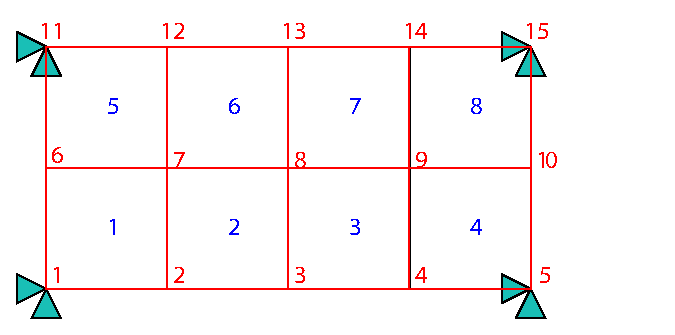
\includegraphics[width=10cm]{fig/problema_calor.eps}
    \caption{Problema depicto en el código \ref{cod:calorDesconocidos}}
    \label{fig:probCalor}
\end{figure}